\section{Part I -- Monovariable Control}\label{sec:part1}

\subsection{Problem Description and Model}\label{sec:prob_descr}

The helicopter test rig has three rotational joints: pitch $p$, elevation $e$ and travel $\lambda$ (\Cref{fig:heli_forces}). Two motors, mounted symmetrically about the pitch axis at distance $l_p$, produce propeller forces $F_f$ and $F_b$ assumed proportional to the applied voltages, $F_f=K_fV_f$ and $F_b=K_fV_b$; only the voltage sum $V_s=V_b+V_f$ and voltage difference $V_d=V_b-V_f$ enter the dynamics. Modelling the motors and the counterweight as point masses and applying $J_\theta\ddot\theta=\sum\tau$ about each axis gives the nonlinear equations of motion \eqref{eq:eom}. Linearising about the equilibrium $p=e=0$ and introducing $\tilde V_s = V_s - V_{s,0}$, chosen such that $\tilde V_s=0$ keeps $e=0$ an equilibrium, yields the decoupled linear model \eqref{eq:lin}. Physical parameters for our helicopter (no.\ 3--10) are listed in \Cref{tab:parameters}; the derived constants $J_p,J_e,J_\lambda,L_1,\ldots,L_4,K_1,K_2,K_3$ and the motor constant $K_f$ follow directly from these and are left as formulas here, since $K_f$ (and hence everything downstream of it) is only pinned down experimentally in Task~2, from the measured $V_{s,0}$. A PD controller \eqref{eq:pd} is used for the pitch loop, giving the closed-loop transfer function \eqref{eq:tf}, whose poles are placed either directly \eqref{eq:kpp_kpd} or via a damping ratio $\zeta$ and natural frequency $\omega_0$ \eqref{eq:kpp_kpd_zeta}; the reasoning behind that choice is discussed below.

\begin{figure}[tp]
	\centering
	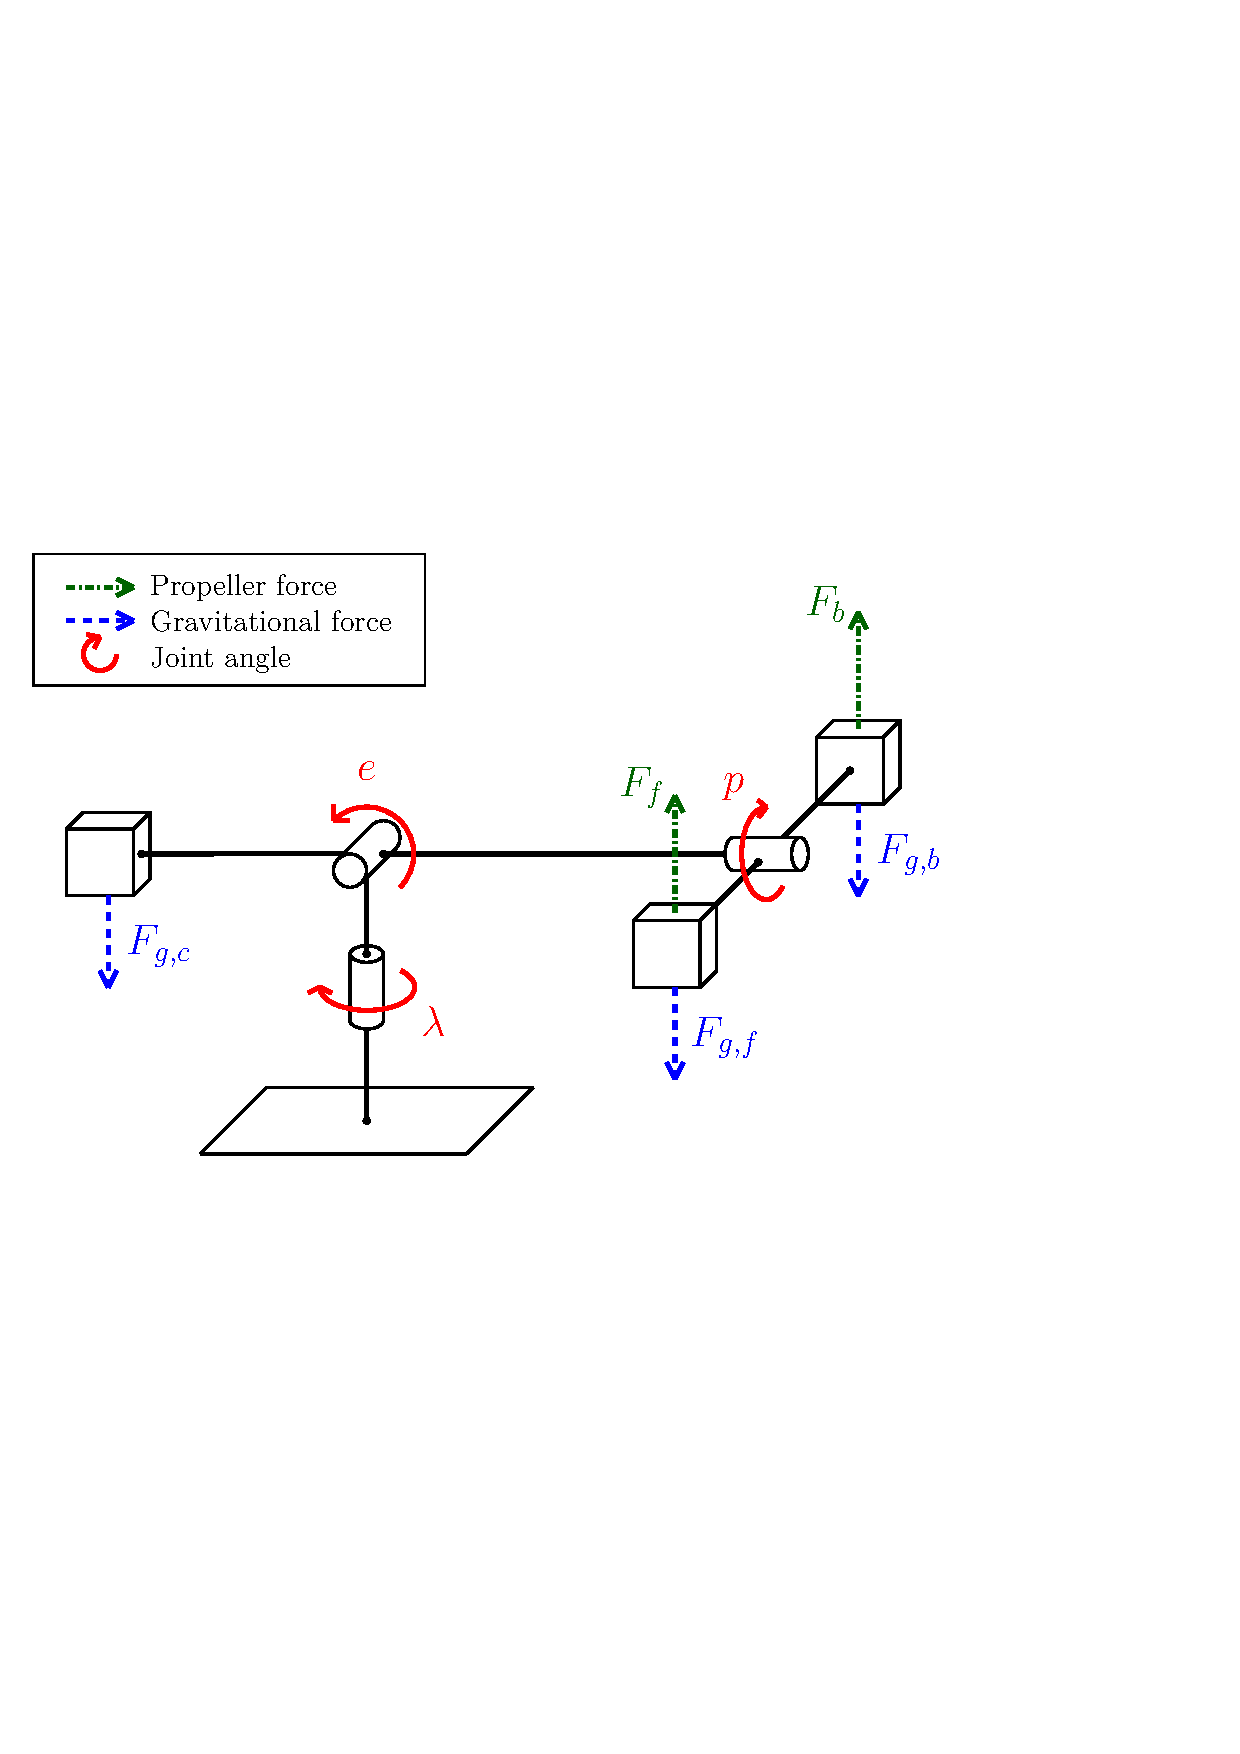
\includegraphics[width=0.85\textwidth]{figures/forces.pdf}
	\caption{Forces and joint angles of the helicopter: pitch $p$, elevation $e$ and travel $\lambda$. Source: TTK4115 Helicopter Lab Assignment, NTNU.}
\label{fig:heli_forces}
\end{figure}

\begin{subequations}\label{eq:eom}
	\begin{align}
		J_p\ddot{p} &= L_1 V_d \\
		J_e\ddot{e} &= L_2\cos(e) + L_3 V_s\cos(p) \\
		J_\lambda\ddot{\lambda} &= L_4 V_s\cos(e)\sin(p)
	\end{align}
\end{subequations}
with
\begin{equation}\label{eq:L_defs}
	L_1 = l_pK_f, \qquad L_2 = g(m_cl_c-2m_pl_h), \qquad L_3=L_4=l_hK_f.
\end{equation}

Requiring $e=0$ to remain an equilibrium point when $\tilde V_s=0$ gives $L_2+L_3V_{s,0}=0$, i.e.\ $V_{s,0}=-L_2/L_3$. Substituting and linearising about $p=e=0$ then yields the decoupled linear model
\begin{subequations}\label{eq:lin}
	\begin{align}
		\ddot{p} &= K_1 V_d, & K_1 &= L_1/J_p, \label{eq:lin_pitch}\\
		\ddot{e} &= K_2 \tilde{V}_s, & K_2 &= L_3/J_e, \label{eq:lin_elev}\\
		\ddot{\lambda} &= K_3 p, & K_3 &= -L_2/J_\lambda, \label{eq:lin_travel}
	\end{align}
\end{subequations}
where $K_3$ is notably independent of $K_f$, since $L_3=L_4$ cancels out of $V_{s,0}$. Since $V_{s,0}=-L_2/L_3$ also depends on $K_f$, it cannot be evaluated from \Cref{eq:L_defs} alone; instead $V_{s,0}$ is measured directly (the voltage sum that holds $e=0$ in steady state), and this measurement is used to solve \Cref{eq:L_defs} for $K_f$, which in turn fixes $J_p,J_e,J_\lambda,L_1,\ldots,L_4,K_1,K_2,K_3$ for the remainder of the lab.

\begin{table}[tbp]
	\centering
	\caption{Physical parameters (helicopter no.\ 3--10) and quantities determined experimentally.}
	\begin{tabular}{llll}
		\toprule
		Symbol & Description & Value & Unit \\
		\midrule
		$g$   & Gravitational acceleration                     & $9.81$   & m/s$^2$ \\
		$l_c$ & Elevation axis to counterweight                & $0.46$   & m \\
		$l_h$ & Elevation axis to helicopter head              & $0.66$   & m \\
		$l_p$ & Pitch axis to motor                             & $0.175$  & m \\
		$m_c$ & Counterweight mass                              & $1.92$   & kg \\
		$m_p$ & Motor mass                                       & $0.72$   & kg \\
		\midrule
		$e_0$     & Elevation encoder offset (measured, Task~2)        & $0.528$  & rad \\
		$V_{s,0}$ & Equilibrium voltage sum (measured, Task~2)         & $7.0$    & V \\
		\bottomrule
	\end{tabular}
\label{tab:parameters}
\end{table}

A PD controller is used to control the pitch angle,
\begin{equation}\label{eq:pd}
	V_d = K_{pp}(p_c-p) - K_{pd}\dot{p},
\end{equation}
where $p_c$ is the joystick reference. Substituting \eqref{eq:pd} into \eqref{eq:lin_pitch} and taking the Laplace transform gives the closed-loop transfer function
\begin{equation}\label{eq:tf}
	G(s) = \frac{P(s)}{P_c(s)} = \frac{K_1K_{pp}}{s^2 + K_1K_{pd}\,s + K_1K_{pp}} =: \frac{K_1K_{pp}}{D(s)}.
\end{equation}

Matching $D(s)$ against the desired closed-loop poles $\lambda_1,\lambda_2$, i.e.\ $D(s)=(s-\lambda_1)(s-\lambda_2)$, gives
\begin{subequations}\label{eq:kpp_kpd}
	\begin{align}
		K_{pd} &= -\frac{\lambda_1+\lambda_2}{K_1}, & K_{pp} &= \frac{\lambda_1\lambda_2}{K_1}.
	\end{align}
\end{subequations}

\paragraph{Why parametrise by $\zeta,\omega_0$ instead of $\lambda_1,\lambda_2$ directly.}
In practice we instead parametrise $D(s)$ by a damping ratio $\zeta$ and a natural frequency $\omega_0$, as in \texttt{init\_heli\_3\_10.m}. This follows by comparing $D(s)=s^2+K_1K_{pd}\,s+K_1K_{pp}$, term by term, with the standard second-order characteristic polynomial $s^2+2\zeta\omega_0\,s+\omega_0^2$: matching the constant terms gives $K_1K_{pp}=\omega_0^2$, and matching the linear-in-$s$ terms gives $K_1K_{pd}=2\zeta\omega_0$, i.e.
\begin{subequations}\label{eq:kpp_kpd_zeta}
	\begin{align}
		K_{pp} &= \frac{\omega_0^2}{K_1}, & K_{pd} &= \frac{2\zeta\omega_0}{K_1}.
	\end{align}
\end{subequations}
This parametrisation is preferred over specifying $\lambda_1,\lambda_2$ directly for three reasons. First, $\lambda_1,\lambda_2$ are only real for $\zeta\geq1$; every underdamped case in our test-plan (\Cref{sec:part1_testplan}) has a complex-conjugate pole pair, so choosing $\lambda_{1,2}$ directly would mean specifying a complex number by hand for most tests, whereas $(\zeta,\omega_0)$ are two real numbers that sweep continuously from underdamped through critically damped to overdamped without any special-casing. Second, $\zeta$ and $\omega_0$ separate \emph{how oscillatory} the response is from \emph{how fast} it is, and connect directly to the standard second-order step-response quantities (overshoot, settling time) that the assignment explicitly asks us to hypothesise about (damped, oscillatory, aggressive, saturating); $\lambda_1,\lambda_2$ affect $K_{pp}$ and $K_{pd}$ jointly through their sum and product, which is far less intuitive to reason about before a test. Third, allowing $\zeta<0$ in \eqref{eq:kpp_kpd_zeta} is a deliberate, single-parameter way to place a pole in the right half-plane and produce a controlled instability, which we use in Task~3 to probe the boundary between theory and the physical (saturating) system.

\subsection{Hypothesis and Test Plan}\label{sec:part1_testplan}
\todo{To be written: hypotheses and test plan for Task 1--3 (see \texttt{Del1\_Plan\_og\_testplan.md} for the working draft).}

\subsection{Results and Discussion}\label{sec:part1_results}
\todo{To be written after post-processing the logged data (\texttt{Task 1-1/data}, \texttt{Task 1-4/data}).}
